%*******************************************************
% Capitulo seis
%*******************************************************

\chapter{Capa de negocio}

\marginpar{
    \begin{figure}[H]
        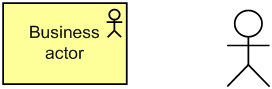
\includegraphics[scale=0.6]{IBusiness_actor}
    \end{figure} 
    \footnotesize 
    \textbf{Actor}. Una entidad organizacional que es capaz de ejecutar un comportamiento.
\newline
}
\marginpar{
    \begin{figure}[H]
        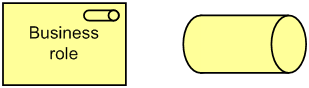
\includegraphics[scale=0.6]{IBusiness_role}
    \end{figure} 
    \footnotesize 
    \textbf{Rol}. La responsabilidad de llevar a cabo un comportamiento específico, al que se le puede asignar un actor.
\newline    
}
\marginpar{
    \begin{figure}[H]
        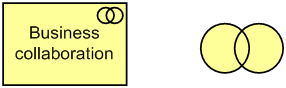
\includegraphics[scale=0.6]{IBusiness_collaboration}
    \end{figure} 
    \footnotesize 
    \textbf{Colaboración}.Un agregado de dos o más funciones de negocios que trabajan en conjunto para llevar a cabo un comportamiento colectivo.
}

\section{Organización}

El punto de vista de organización se centra en la organización de una empresa, un departamento, una red de empresas o cualquier otra entidad organizativa. Es posible presentar los modelos de este punto de vista como diagramas de bloques anidados o de una manera mas tradicional a través de un organigrama. Este punto de vista es muy útil en la identificación de las competencias, la autoridad y las responsabilidades dentro de la organización. 


\begin{figure}[h]
\centering
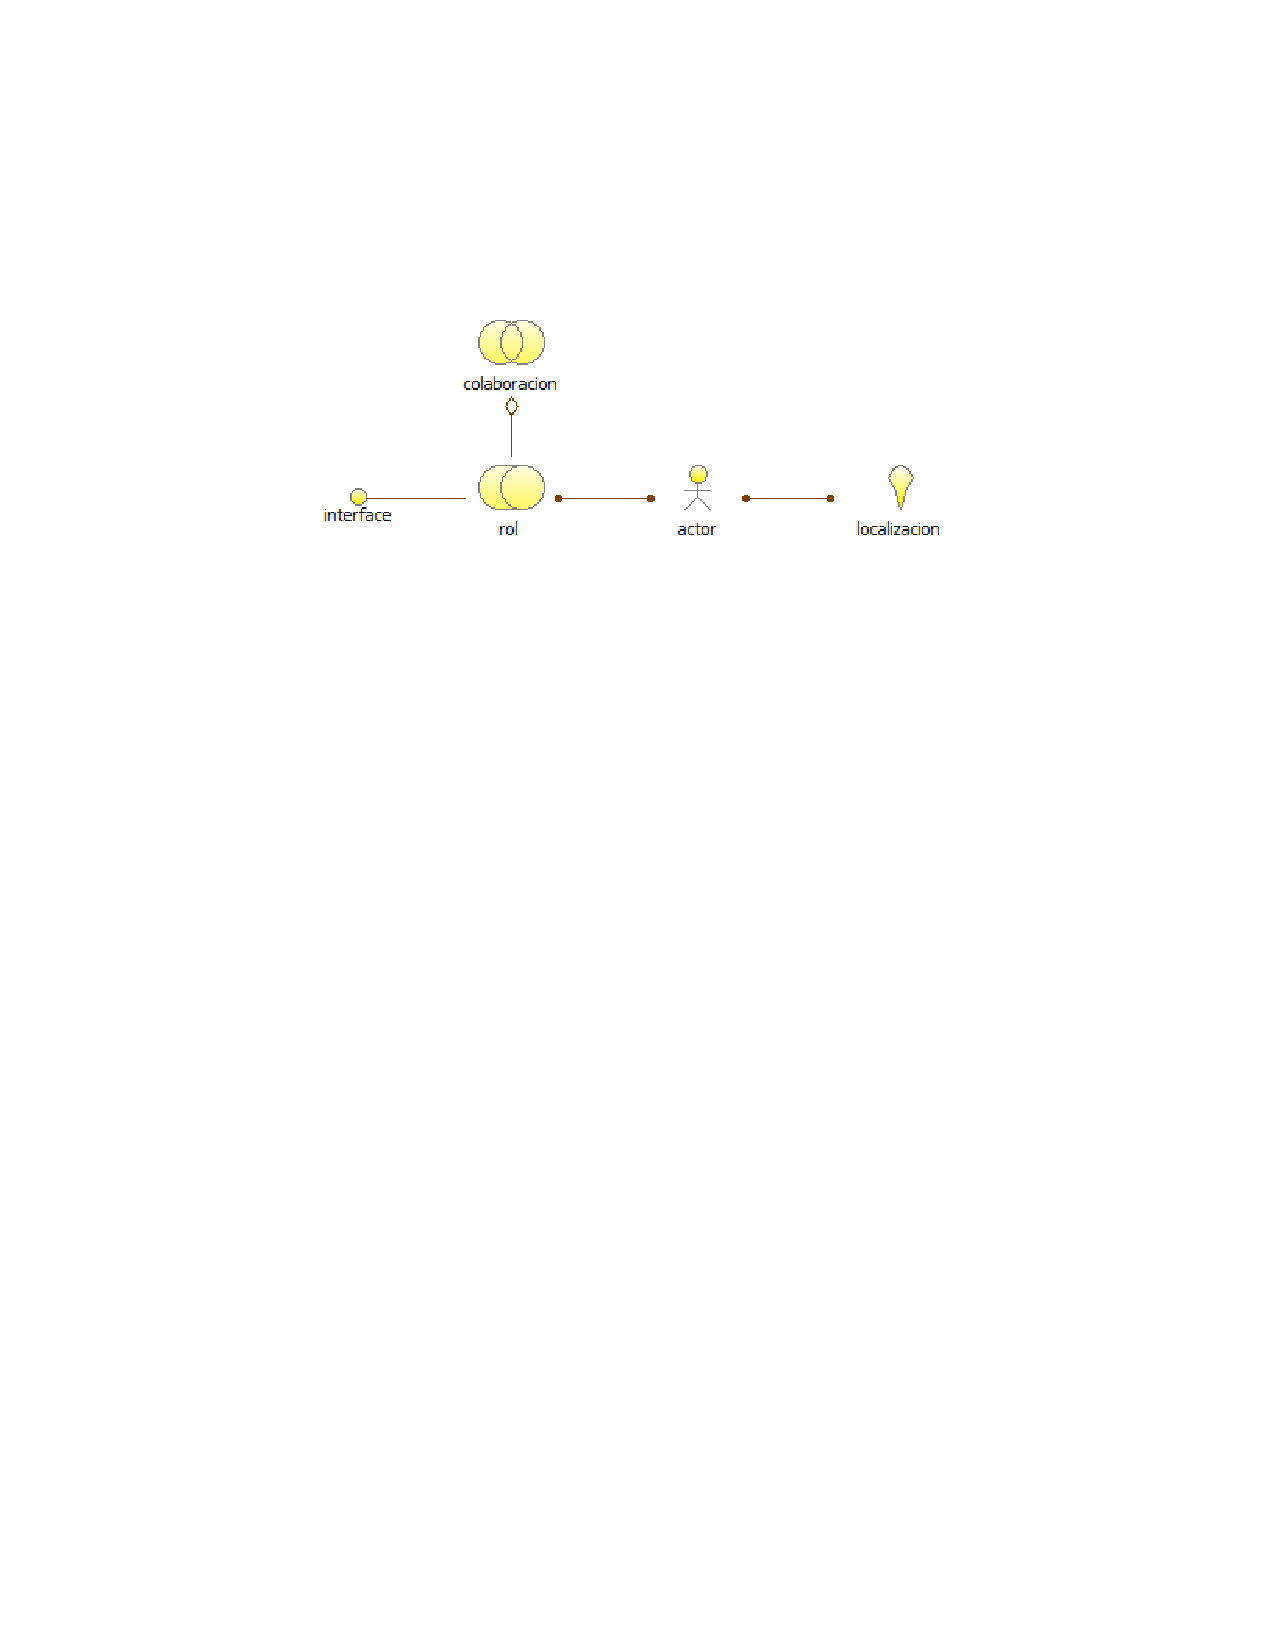
\includegraphics{organizacion}
\caption{Metamodelo del punto de vista organización.}
\end{figure}

En función del cumplimiento de los objetivos planteados, se propone la siguiente estructura organizacional para desarrollar el negocio.

\begin{figure}[h]
\centering
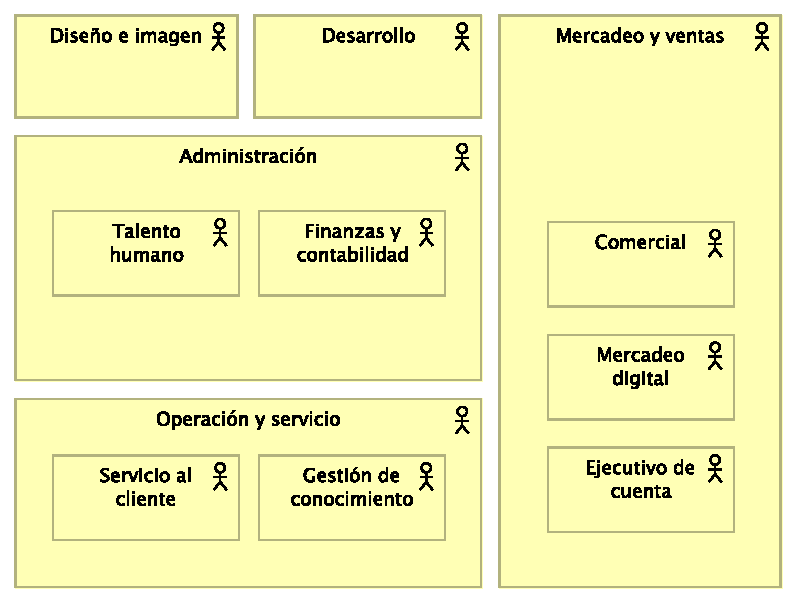
\includegraphics{Morganizacion}
\caption{Punto de vista organización.}
\end{figure}
 
\section{Cooperación de actor}

\marginpar{
    \begin{figure}[H]
        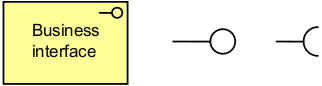
\includegraphics[scale=0.6]{ibusiness_interfaz}
    \end{figure} 
    \footnotesize 
    \textbf{Interfaz}.Un punto de acceso donde se pone a disposición un servicio de negocio para el entorno.
\newline
}
\marginpar{
    \begin{figure}[H]
        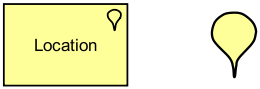
\includegraphics[scale=0.6]{ilocacion}
    \end{figure} 
    \footnotesize 
    \textbf{Ubicación}. Un lugar conceptual en el espacio.
\newline    
}


El punto de vista de cooperación de actor se centra en las relaciones de los actores entre sí y con su entorno. Un ejemplo común de esto es el "diagrama de contexto", lo que pone una organización con su entorno, que consiste en las partes externas, tales como clientes, proveedores y otros socios comerciales.Es muy útil en la determinación de dependencias externas y colaboraciones y muestra la cadena de valor o de la red en el que opera el actor. 

Otro uso importante es mostrar cómo una serie de actores comerciales y/o componentes de la aplicación en conjunto cooperan para realizar un proceso de negocio. Por lo tanto, en este punto de vista,le puede aplicar tanto a los actores comerciales o funciones y a los componentes de la aplicación.

\begin{figure}[h]
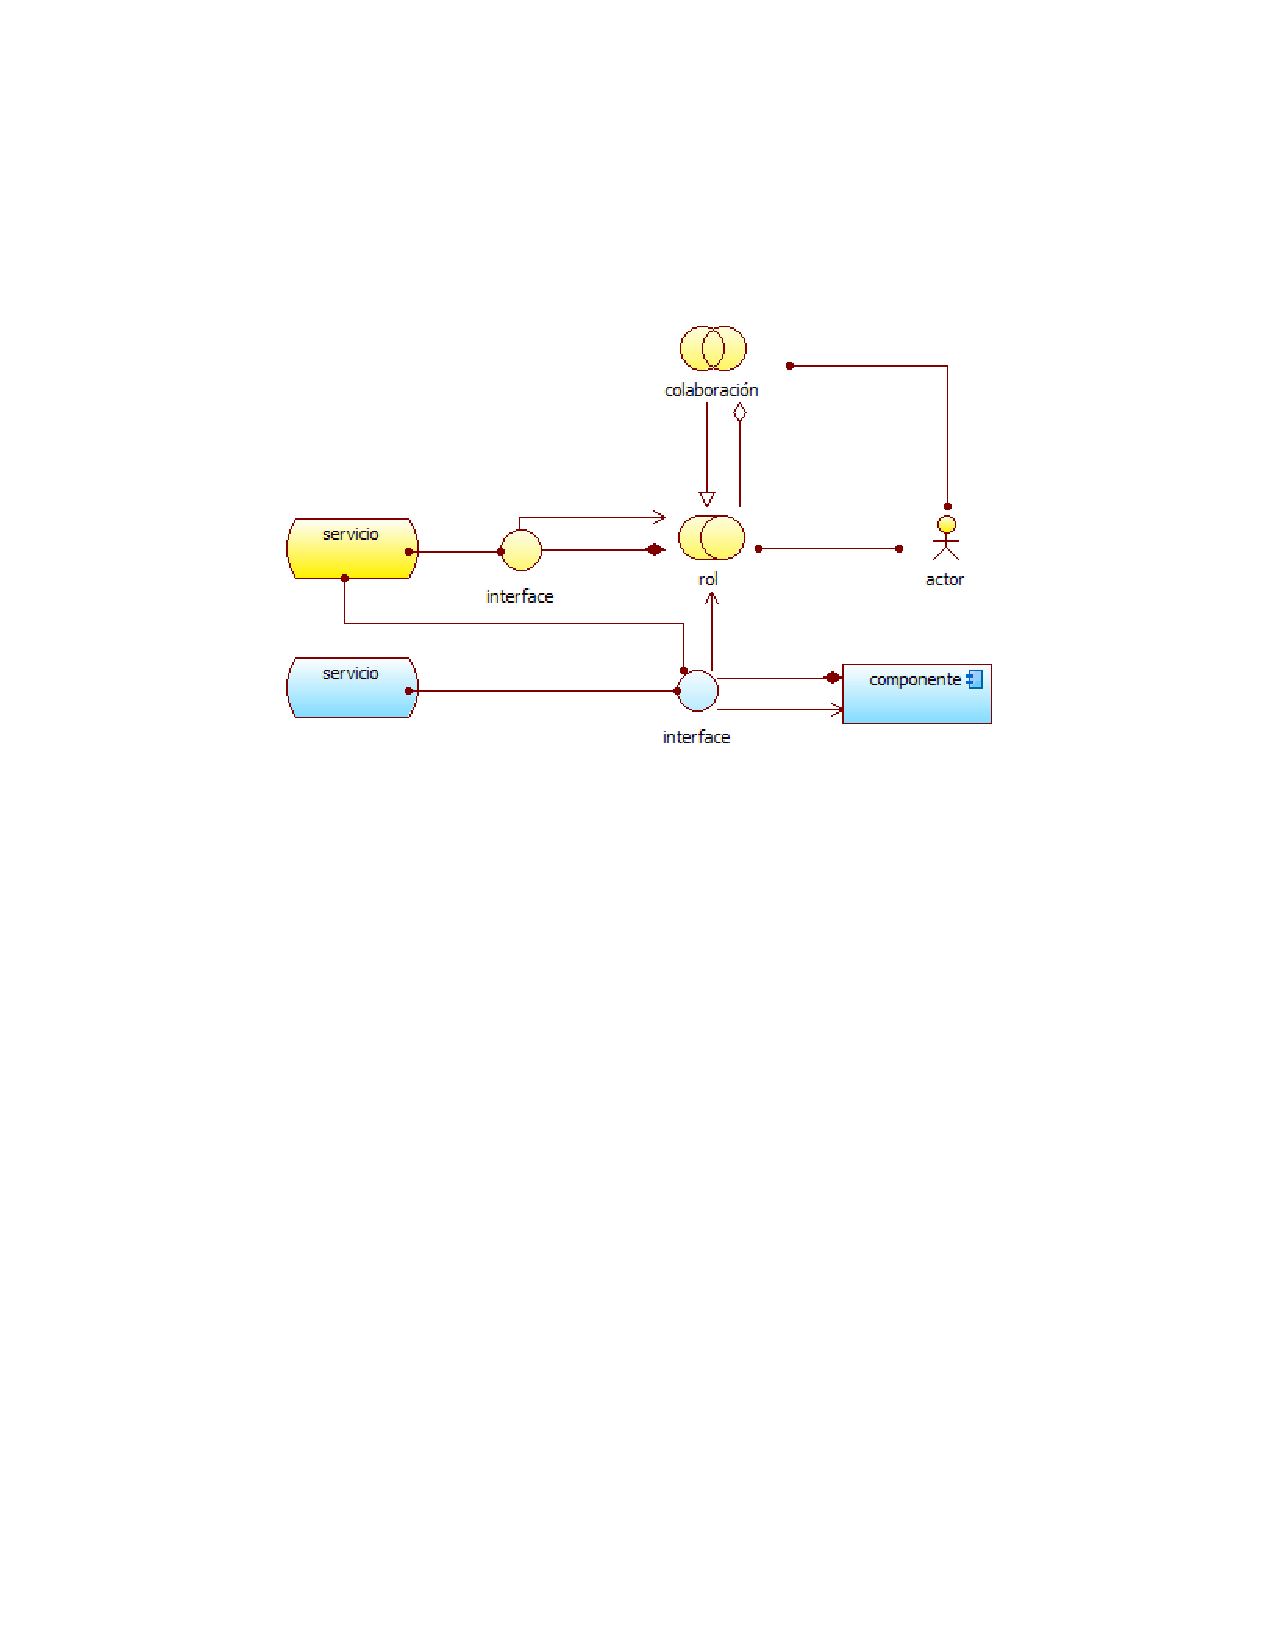
\includegraphics[scale=0.7]{cooperacion}
\centering
\caption{Metamodelo del punto de vista de cooperación de Actor.}
\end{figure}

Los stakeholders clave mantienen una relación con la estructura organizacional que se puede observar en la figura \ref{mcooperacionactor}.

\begin{figure}[h] 
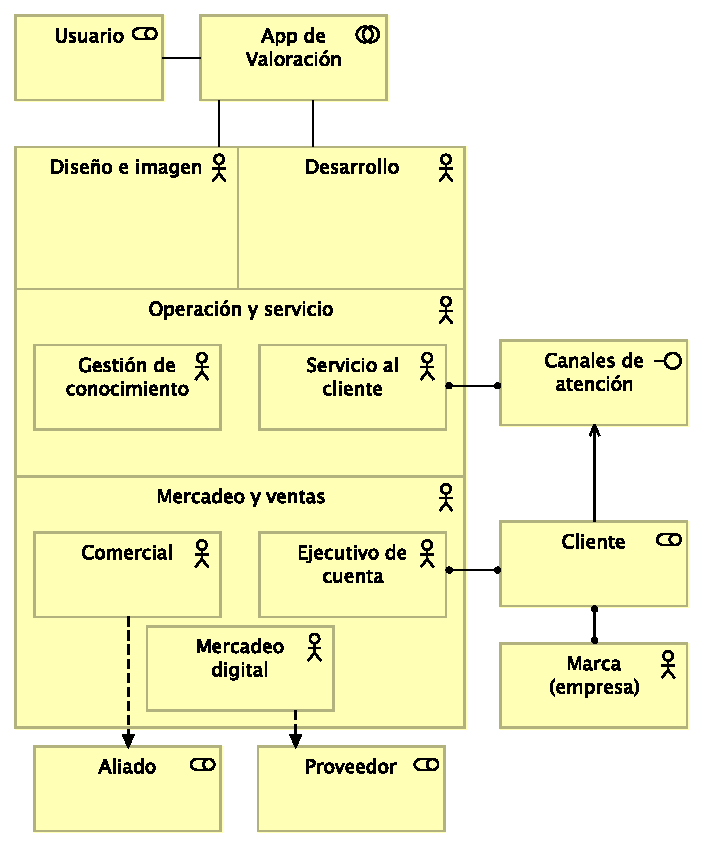
\includegraphics[scale=0.7]{Mcooperacionactor}
\centering
\caption{Punto de vista de cooperación de Actor.}
\label{mcooperacionactor}
\end{figure}

\section{Función de negocio}

\marginpar{
    \begin{figure}[H]
        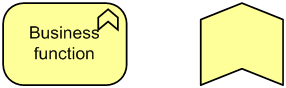
\includegraphics[scale=0.6]{ibusiness_funcion}
    \end{figure} 
    \footnotesize 
    \textbf{Función}. Un elemento de comportamiento que agrupa comportamientos basado en un conjunto seleccionado de criterios (por lo general requiere recursos de la empresa y/o competencias).
\newline
}El punto de vista de funciones de negocios muestra las principales funciones de negocio de una organización y sus relaciones en términos de los flujos de información, el valor, y bienes entre ellos. Este punto de vista es empleado para representar los aspectos más estables de una empresa en términos de las actividades primarias que realiza, independientemente de los cambios de organización o desarrollos tecnológicos. Por lo tanto, la arquitectura función de negocio de las empresas que operan en el mismo mercado a menudo presentan grandes similitudes. De esta manera, el punto de vista de la función empresarial proporciona una visión de alto nivel en las operaciones generales de la empresa, y se puede utilizar para identificar las competencias necesarias, o para estructurar una organización de acuerdo a sus actividades principales. El metamodelo se puede observar en la Figura \ref{funcion_de_negocio}.

\begin{figure}[H]   
\centering
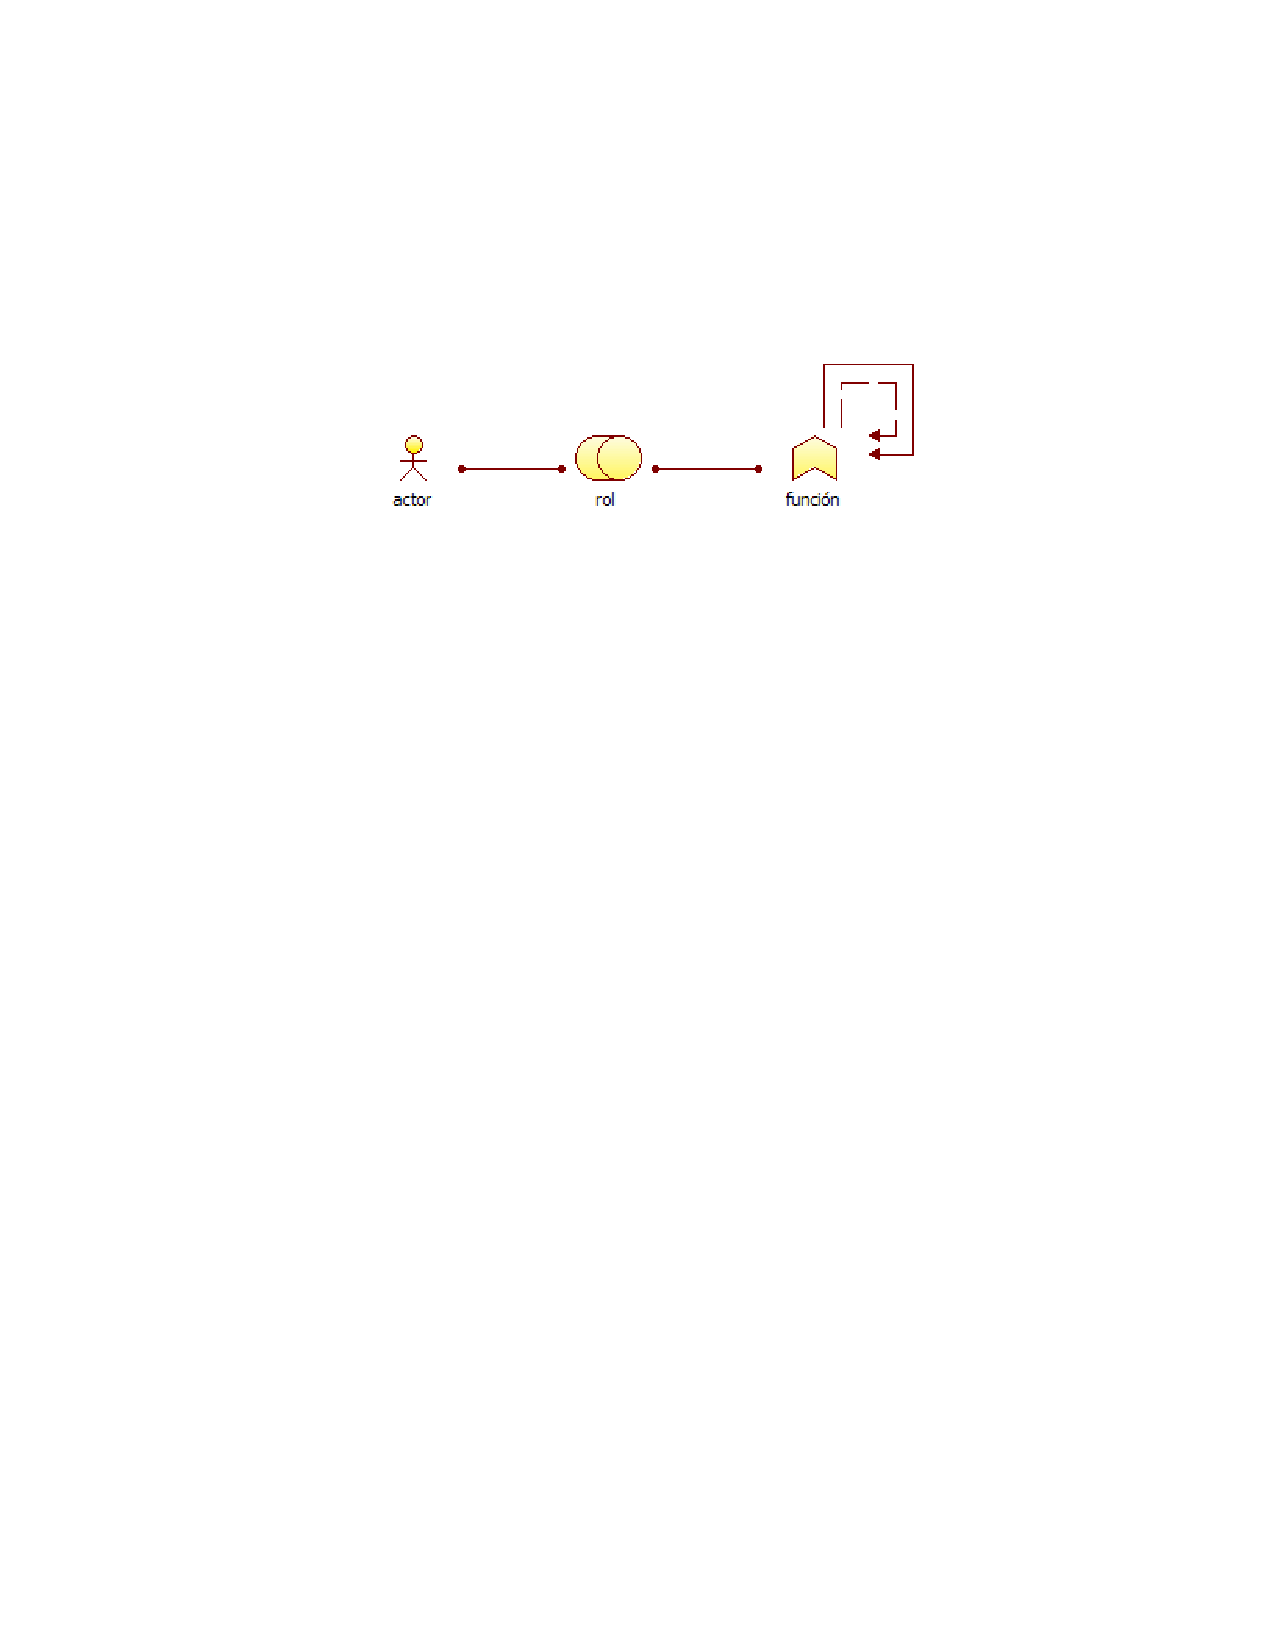
\includegraphics{funcion_de_negocio}
\caption{Metamodelo del punto de vista de función de negocio.}
\label{funcion_de_negocio}
\end{figure}

Como parte de las funciones principales con algunos interesados se tiene la compra de servicios de tecnología como ads de publicidad o servicios de cloud y mantener alto el relacionamiento con los clientes. Esta lista de posibilidades de relación se puede consultar en la descripción canvas del relacionamiento con el cliente.

\begin{figure}[H]   
\centering
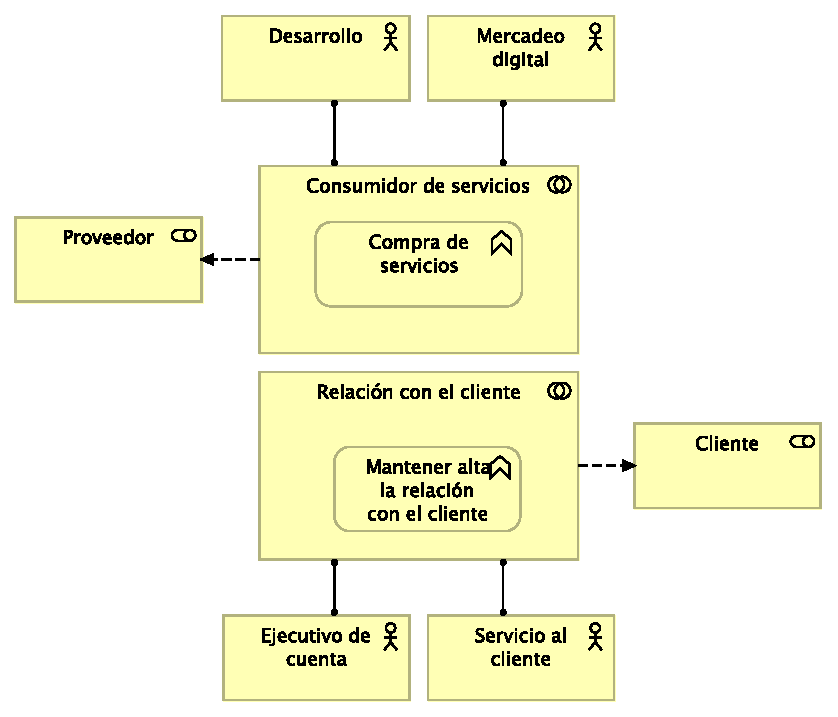
\includegraphics{MFuncionnegocio}
\caption{Punto de vista de función de negocio.}
\label{MFuncionnegocio}
\end{figure}


\section{Proceso de Negocio}


\marginpar{
    \begin{figure}[H]
        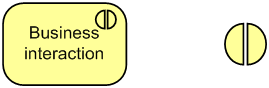
\includegraphics[scale=0.6]{ibusiness_interaccion}
    \end{figure} 
    \footnotesize 
    \textbf{Interacción}.Un elemento de comportamiento que describe el comportamiento de una colaboración.
\newline    
}
El punto de vista de procesos de negocio se utiliza para mostrar una estructura de alto nivel y la composición de uno o más procesos de negocio. Al lado de los mismos procesos, este punto de vista contiene otros conceptos directamente relacionados, como:
\marginpar{
    \begin{figure}[H]
        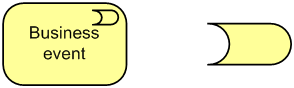
\includegraphics[scale=0.6]{ibusiness_evento}
    \end{figure} 
    \footnotesize 
    \textbf{Evento}.Algo que sucede (interna o externa) e influye en el comportamiento.
    \\
}

\marginpar{
    \begin{figure}[H]
        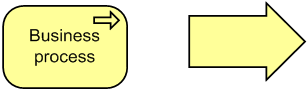
\includegraphics[scale=0.6]{ibusiness_proceso}
    \end{figure} 
    \footnotesize 
    \textbf{Proceso}. Un elemento de comportamiento que agrupa comportamientos basado en un ordenamiento de actividades.
}
\begin{itemize}
        \item Los servicios que ofrece un proceso de negocio con el mundo exterior, que muestra cómo un proceso contribuye a la realización de productos de la compañía.
        \item La asignación de los procesos de negocio a los roles, lo que da una idea de las responsabilidades de los actores asociados.
        \item La información utilizada por el proceso de negocio. 
\end{itemize}
Cada uno de ellos puede ser considerado como un "sub -view" de la vista de procesos de negocio.

\begin{figure}[H]
\centering
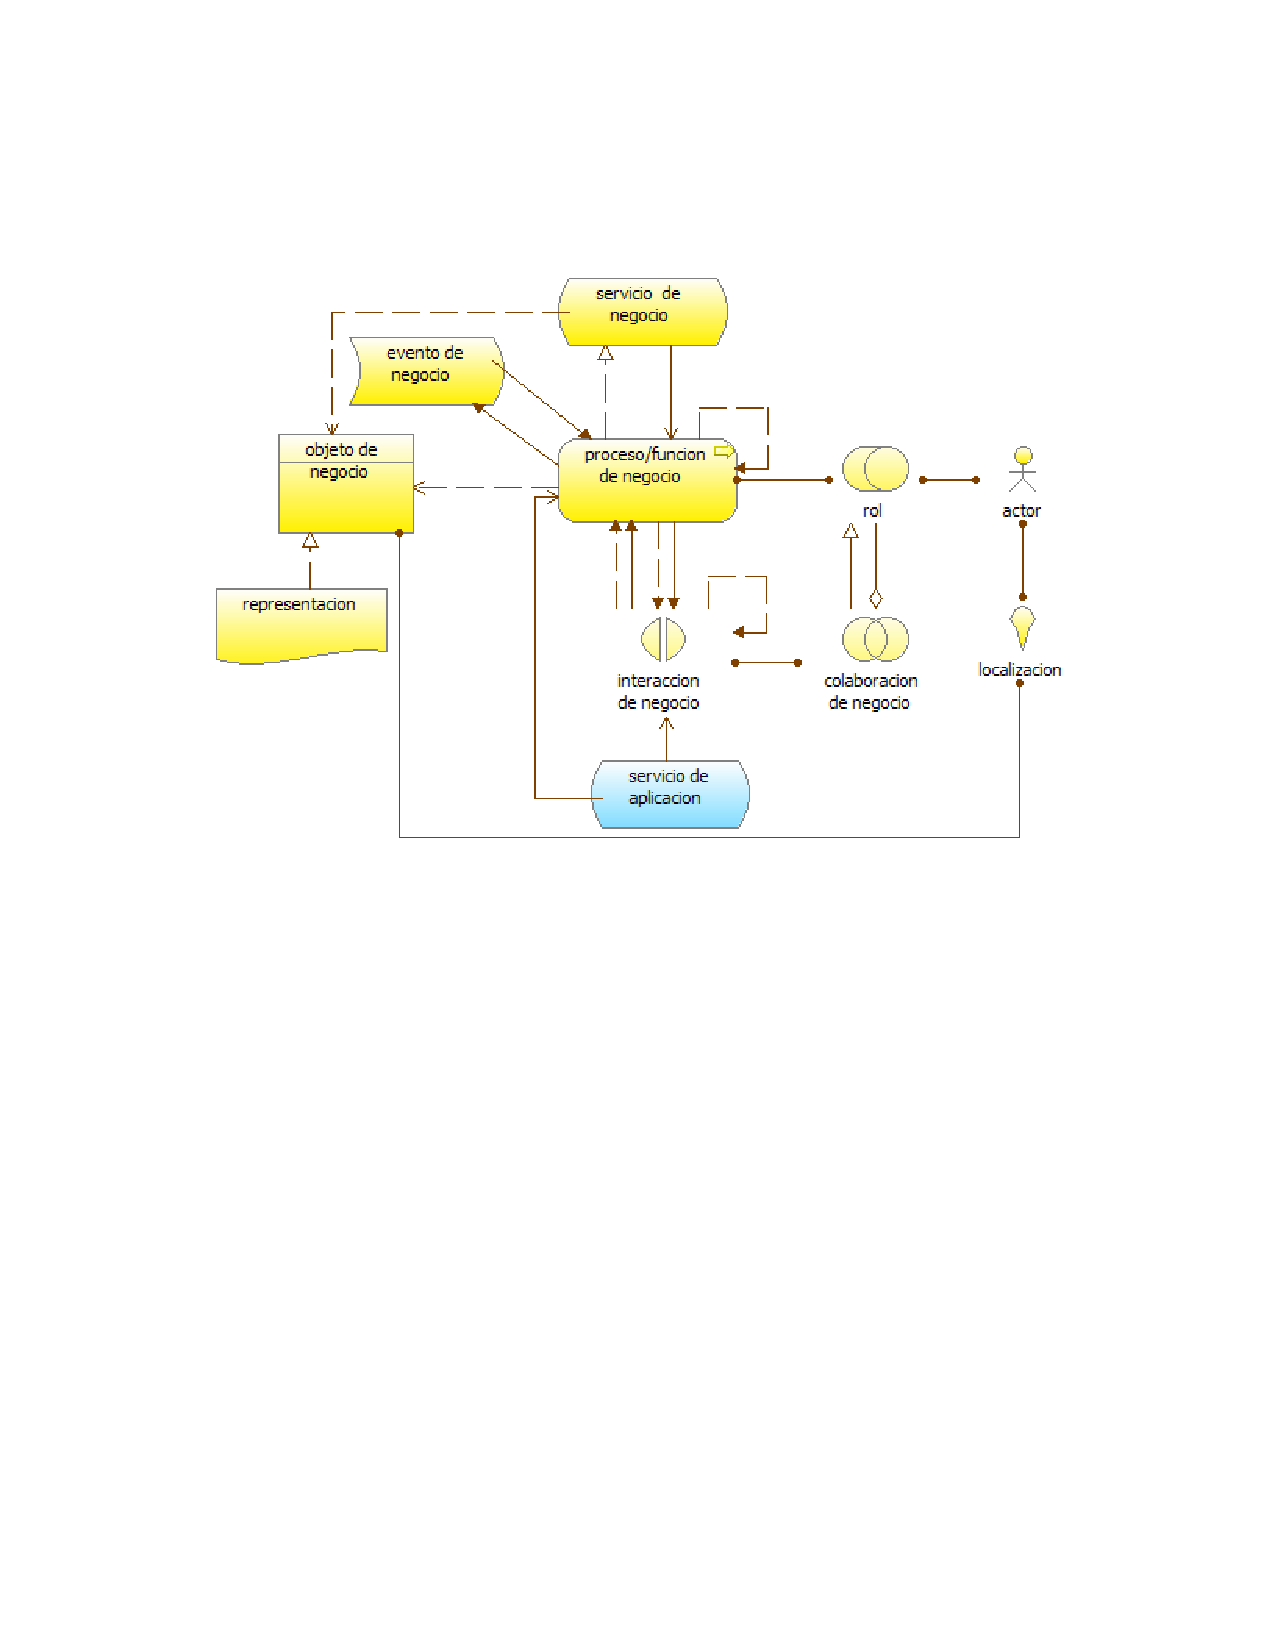
\includegraphics[scale=0.7]{proceso_de_negocio}
\caption{Punto de vista de proceso de negocio.}
\end{figure}

Se plantea entonces para esta propuesta los procesos más importantes frente al uso de la aplicación sin que sean menos relevantes la gestión comercial, el consumo de servicios de tecnología, las actividades de relacionamiento u otras descritas por el canvas. Son las actividades que hacen del uso de la aplicación un factor diferencial en proceso de negocio.

\begin{figure}[H]
\centering
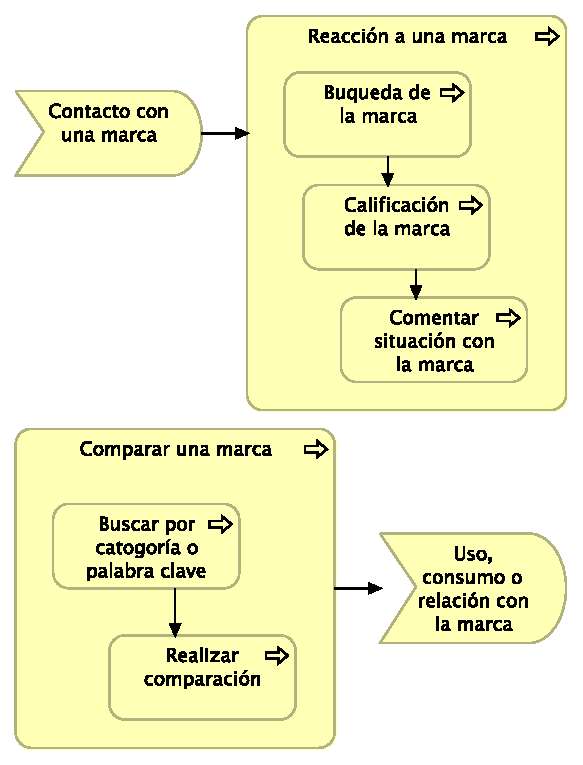
\includegraphics[scale=0.8]{MProcesonegocio}
\caption{Metamodelo del punto de vista de proceso de negocio.}
\end{figure}

\marginpar{
    \begin{figure}[H]
        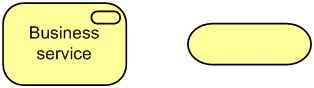
\includegraphics[scale=0.6]{ibusiness_servicio}
    \end{figure} 
    \footnotesize 
    \textbf{Servicio}.Un servicio que satisface una necesidad para un cliente (interno o externo de la organización).
\newline
}
\marginpar{
    \begin{figure}[H]
        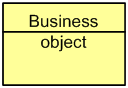
\includegraphics[scale=0.8]{ibusiness_objeto}
    \end{figure} 
    \footnotesize 
    \textbf{Objeto}.Un elemento pasivo que es relevante desde una perspectiva de negocio. 
\newline    
}


\section{Cooperación de proceso de negocio}
El punto de vista de cooperación de proceso de negocio se utiliza para mostrar las relaciones de uno o más procesos de negocio entre sí y/o con su entorno. Puede ser utilizado tanto para crear un diseño de alto nivel de los procesos de negocio dentro de su contexto y para proporcionar un gestor operativo responsable de uno o más de estos procesos con penetración en sus dependencias. Algunos aspectos importantes del proceso de cooperación empresarial son:
\begin{itemize}
        \item Los causales de la relación entre los principales procesos de negocio de la empresa.
        \item Mapeo de los procesos de negocio en las funciones de negocio. 
        \item La realización de los servicios por parte de los procesos de negocio.
        \item El uso de datos compartidos.
\end{itemize}
\marginpar{
    \begin{figure}[H]
        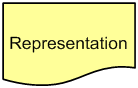
\includegraphics[scale=0.8]{irepresentacion}
    \end{figure} 
    \footnotesize 
    \textbf{Representación}. Una forma perceptible de empaquetado de la información de un objeto de negocio. 
}\marginpar{
    \begin{figure}[H]
        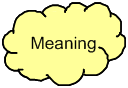
\includegraphics[scale=0.8]{isentido}
    \end{figure} 
    \footnotesize 
    \textbf{Significado}.El conocimiento o experiencia presente en un objeto de negocio o de su representación, dado un contexto particular.
\newline
}Cada uno de ellos puede ser considerado como un "sub -view" de la vista de la cooperación de procesos de negocio.

\begin{figure}[h]
\centering
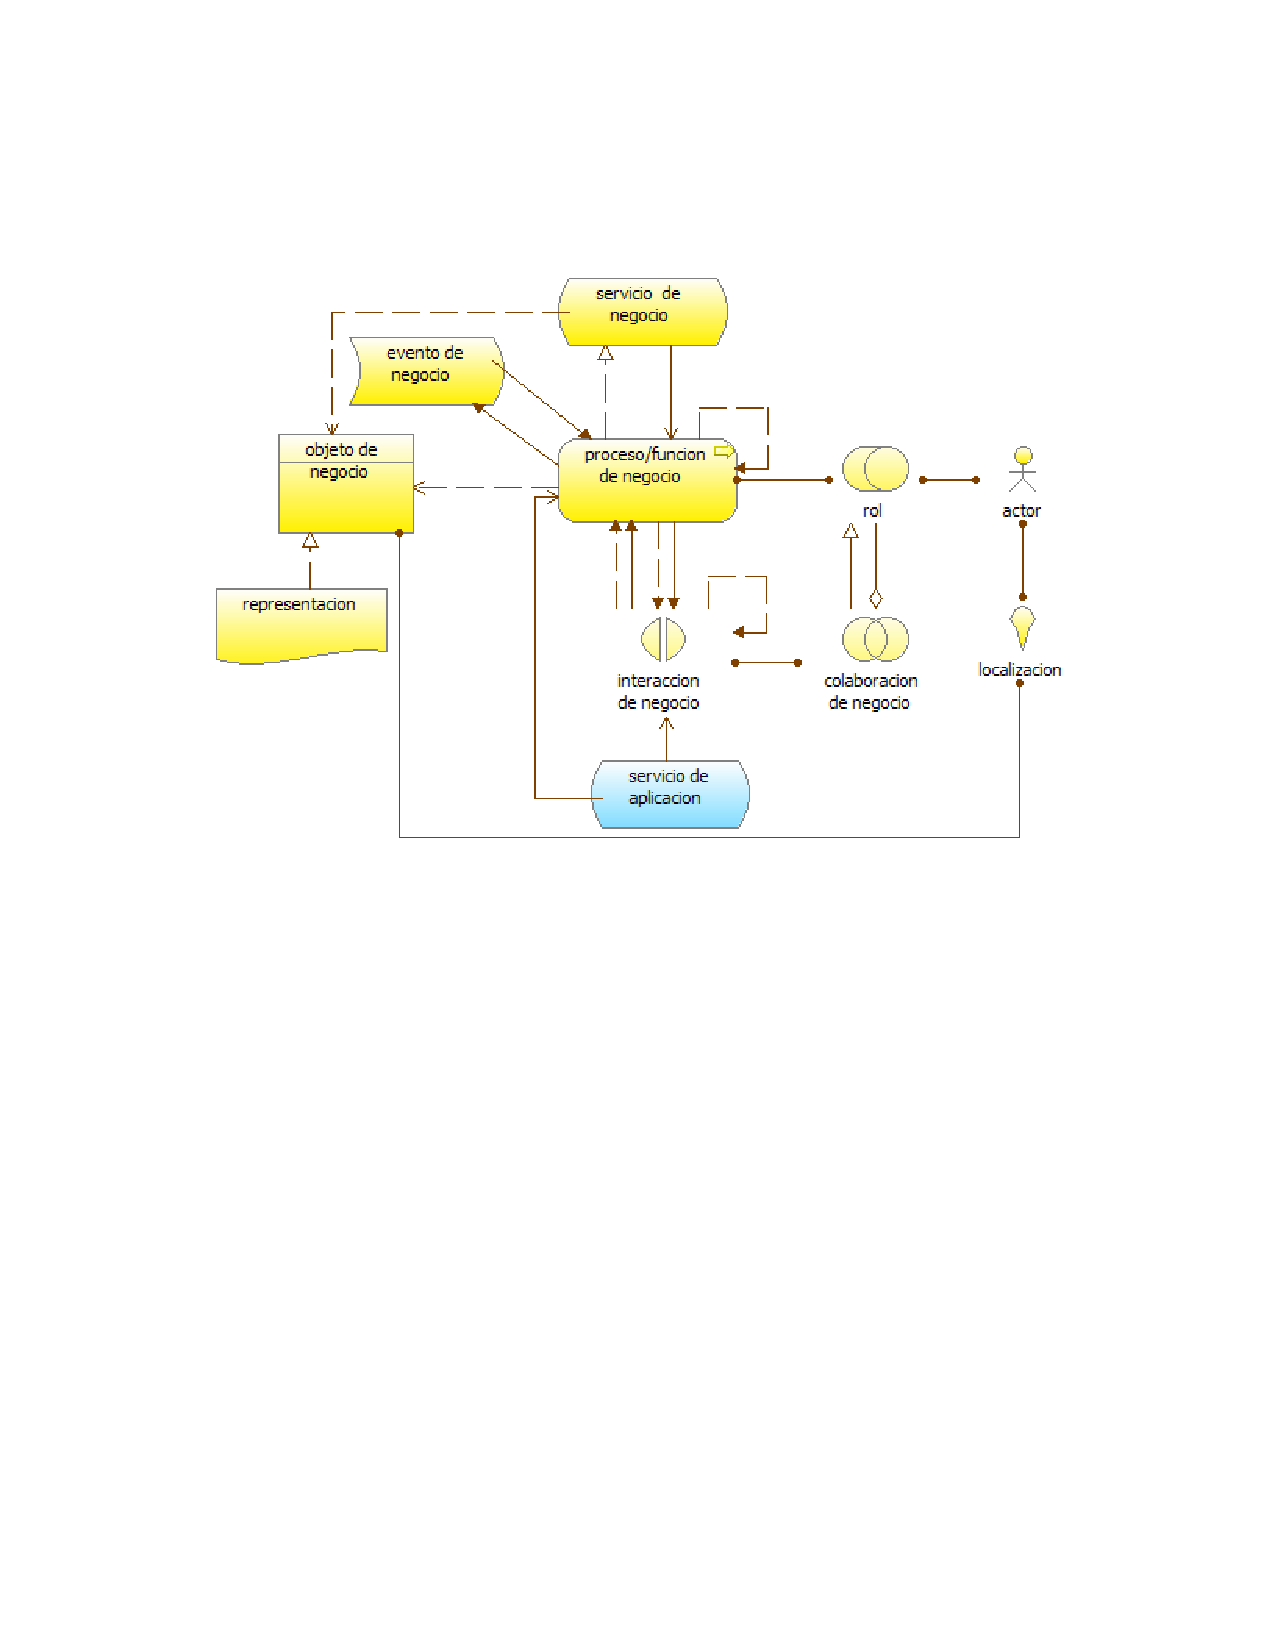
\includegraphics[scale=0.7]{cooperacion_de_proceso_de_negocio}
\caption{Metamodelo del punto de vista de cooperación de proceso de negocio.}
\end{figure}

Los procesos principales al rededor de la aplicación tienen que ver con los eventos en los que se detecta una interacción con una marca y se intenta documentar el resultado de la interacción. Esta información se usa para hacer posteriores comparaciones más adelante y divulgar la información de la gestión. Las marcas deberían reaccionar ante situaciones de percepción negativa y mejorar su calidad.

\begin{figure}[H]
\centering
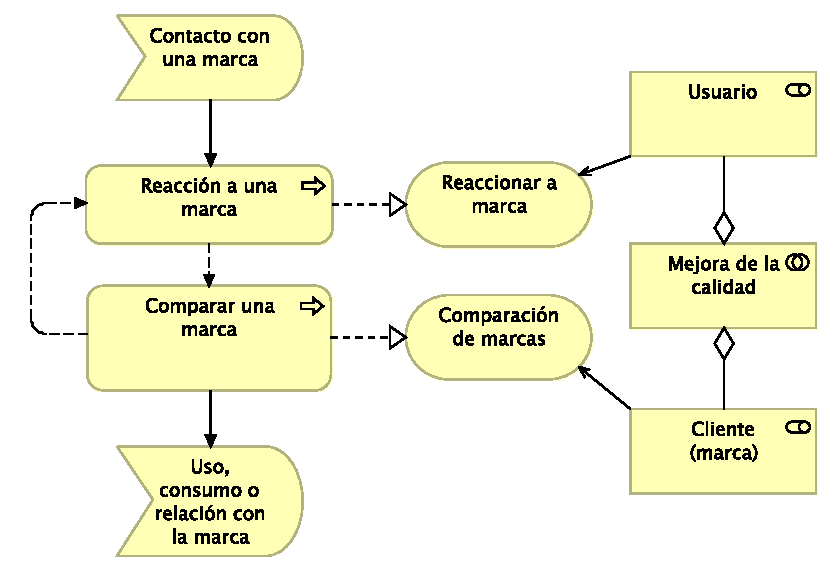
\includegraphics[scale=0.8]{Mcooperacionproceso}
\caption{Punto de vista de cooperación de proceso de negocio.}
\end{figure}

\section{Producto}

\marginpar{
    \begin{figure}[H]
        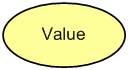
\includegraphics[scale=0.8]{ivalor}
    \end{figure} 
    \footnotesize 
    \textbf{Valor}.El valor relativo, utilidad o importancia de un servicio o producto. 
}\marginpar{
    \begin{figure}[H]
        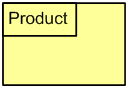
\includegraphics[scale=0.8]{iproducto}
    \end{figure} 
    \footnotesize 
    \textbf{Producto}. Una colección coherente de los servicios, acompañada de un contrato/conjunto de acuerdos, que se ofrece a los clientes (internos o externos). 
\newline
}

El punto de vista del producto representa el valor que estos productos ofrecen a los clientes u otras partes externas involucradas y se muestra la composición de uno o más productos en términos de la constitución (aplicación empresarial o) los servicios, y el contrato(s) asociado u otros acuerdos. 

También puede ser utilizado para mostrar las interfaces (canales) a través de los cuales se ofrece este producto, y los eventos asociados con el producto. El punto de vista del producto se usa frecuentemente en el desarrollo de productos para diseñar un producto mediante la composición de los servicios existentes o mediante la identificación de nuevos servicios que deben ser creados para este producto, dado el valor que un cliente espera. Puede entonces servir como entrada para los arquitectos de procesos de negocios y otros que necesitan para diseñar los procesos y las unidades que realizan estos productos.

\begin{figure}[H]
\centering
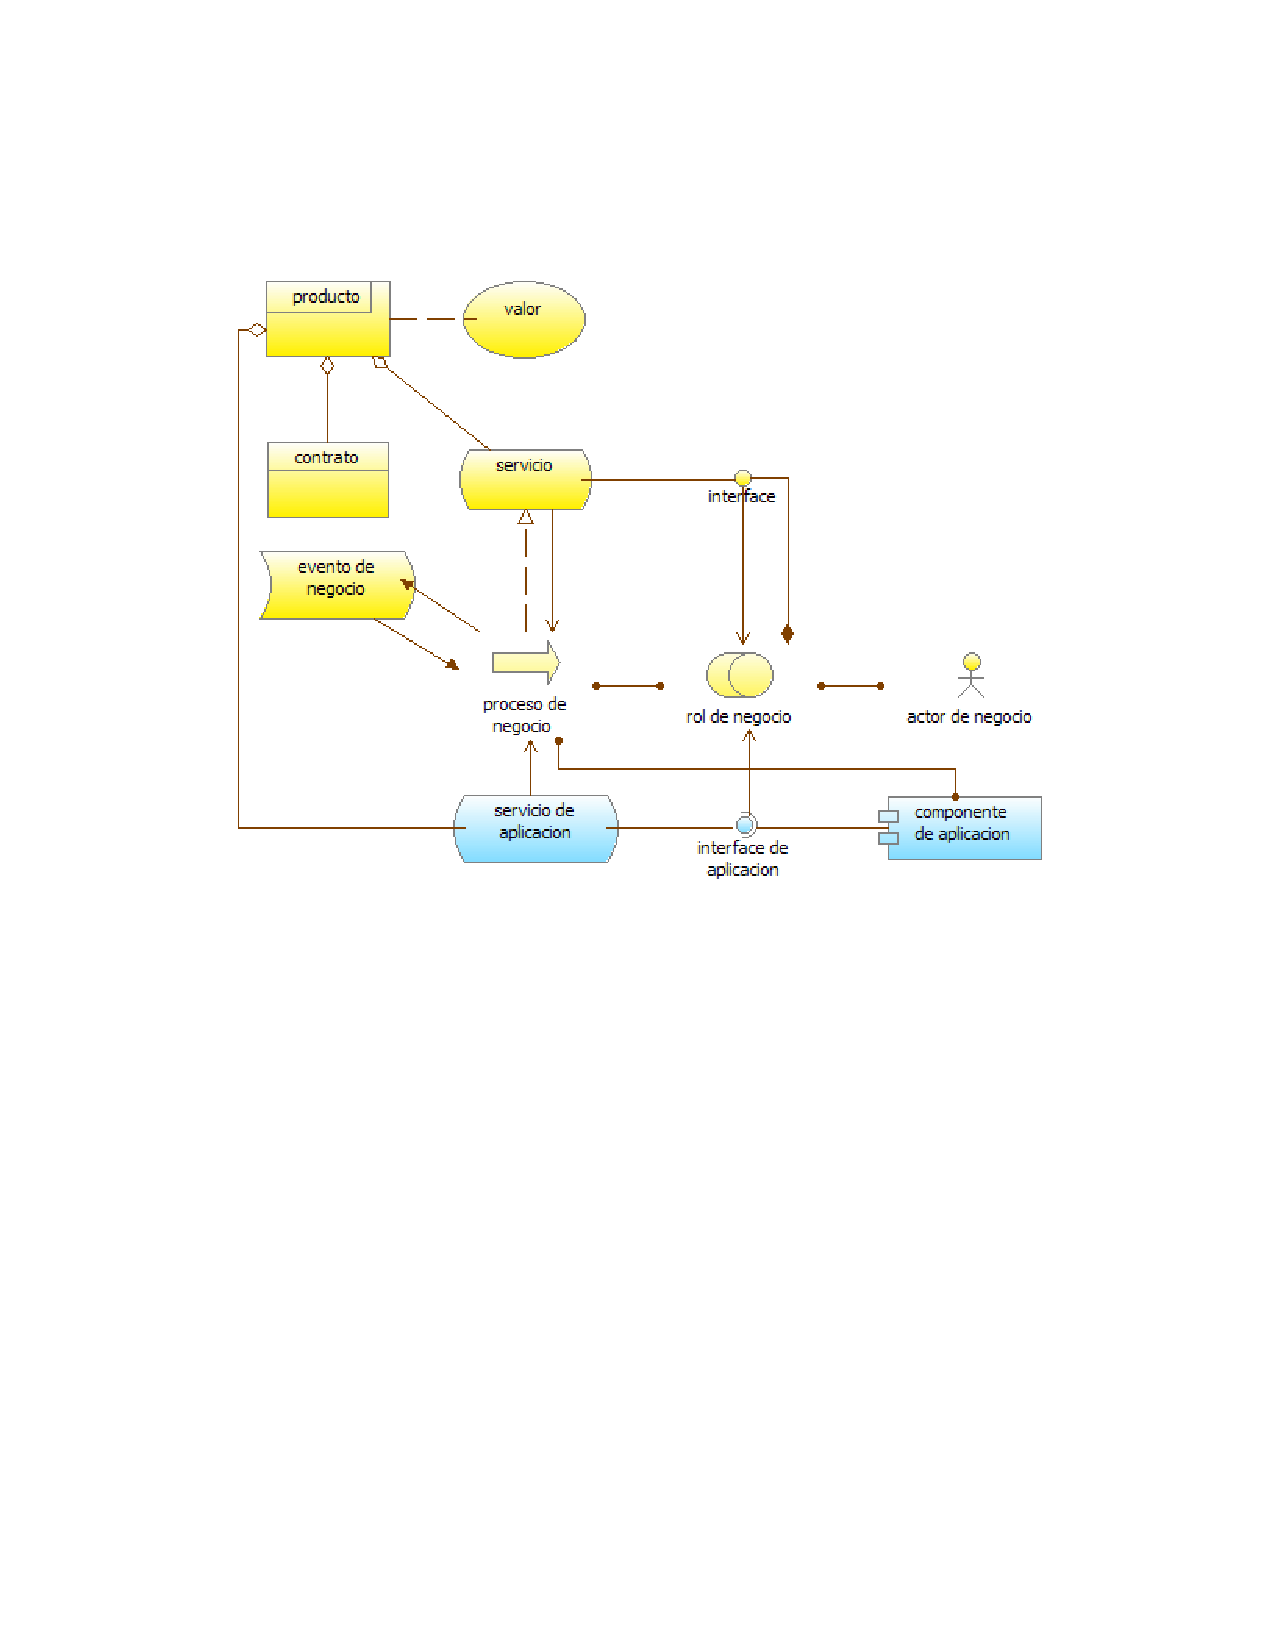
\includegraphics[scale=0.7]{producto}
\caption{Metamodelo del punto de vista de producto.}
\end{figure}


\marginpar{
    \begin{figure}[H]
        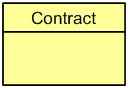
\includegraphics[scale=0.8]{icontrato}
    \end{figure} 
    \footnotesize 
    \textbf{Contrato}.Una especificación formal o informal de acuerdo que especifica los derechos y obligaciones inherentes a un producto. 
}

El producto actual está caracterizado por dos formas de negocio que suplen las condiciones de valor presentadas con el modelo canvas. La primera la aplicación móvil para los usuarios en donde pueden desarrollar servicios específicos generando valor de compartir información y con el impacto de la mejora de la calidad entre las marcas.

\begin{figure}[H]
\centering
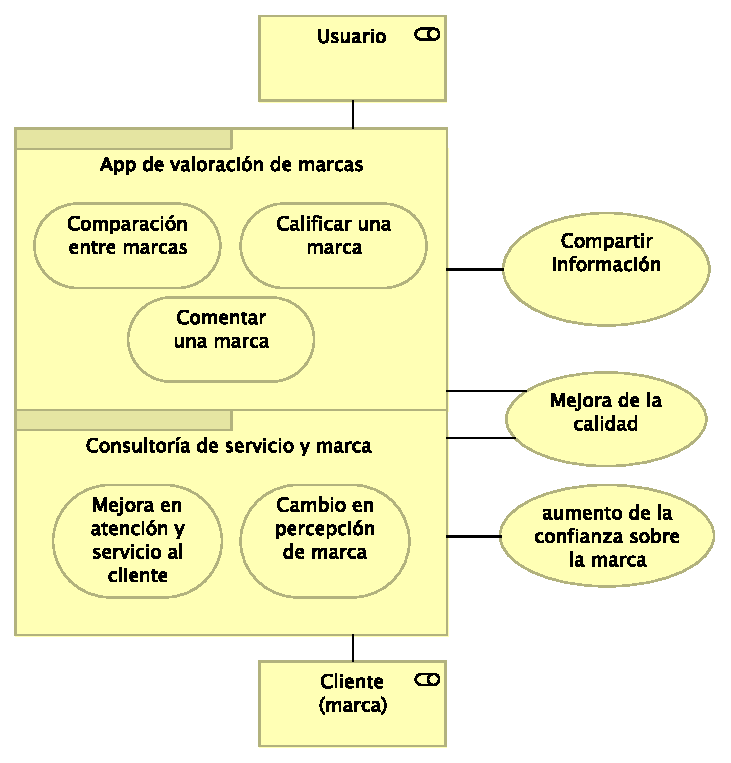
\includegraphics[scale=0.9]{Mproducto}
\caption{Punto de vista de producto.}
\end{figure}

